Verschiebt man ein kontinuierliches Streifenmuster entlang seiner Ausbreitungsrichtung, dann kann man eine \textit{Periodizität} feststellen.
Daraus lässt sich dann für solche Streifenmuster der Begriff der \textit{Phase} ableiten.
Die Phase eines Streifenmusters lässt sich dabei definieren als die aktuelle Position der Streifen im Ablauf dieses periodischen Vorgangs.
Die verschiedenen Streifenmuster sind somit voneinander \textit{phasenverschoben}.
Die Phase wird durch einen Phasenwinkel angegeben, welcher von $ 0 $ bis $ 2\pi $ läuft.
Eine Verschiebung um $ \pi $ bedeutet dementsprechend eine Phasenverschiebung um die halbe Periode.
Anschaulich stellt man fest, dass für gleich breite helle und dunkle Streifen diese ihre Positionen tauschen.
Dies kann man sich zunutze machen, denn das bedeutet, dass die Schnittmenge der dunklen Streifen in den beiden Streifenmustern am kleinsten ist.
Da bestimmte Fehlstellen entweder in den dunklen oder in den weißen Streifen deutlich zu erkennen sind, ergänzen sich die beiden Streifenmuster in ihrer Information.
Verknüpft man die Kamerabilder von solchen Mustern, dann kann man damit die meiste Information aus zwei Bildern extrahieren.
Durch zusätzliche Bildaufnahmen mit verschobenen Streifenmustern kann man detailliertere Oberflächeninformationen von dem Prüfobjekt gewinnen.

\begin{figure}[H]
	\centering
	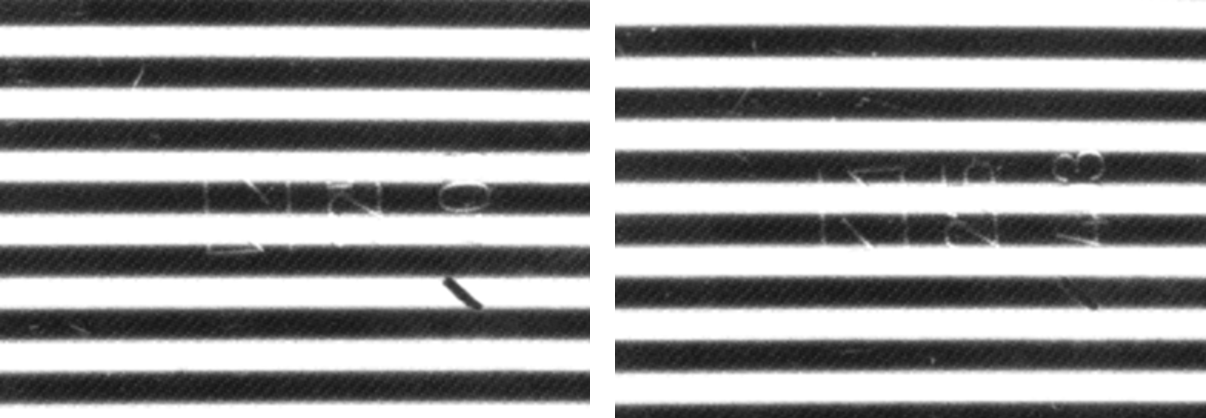
\includegraphics[width=\textwidth]{03_sichtpruefungDurchLichtstreuung/einsatzVonMehrerenStreifenmustern/figures/imageToLink}
	\caption[Zu verknüpfende Bilder]{Kameraaufnahme eines Prüfobjekts unter Projektion von Streifenmustern mit einer Phasenverschiebung von $ \pi $ zueinander.}
	\label{img:imageToLink}
\end{figure}

\noindent
Wie man erkennt, sind die Streifen der beiden Bilder genau voneinander versetzt.
Damit ist auch die erfasste Information möglichst versetzt, das heißt, dass die beiden Bilder sich in ihrer Oberflächeninformation ergänzen.
Zur Verknüpfung der Information in einem Gesamtbild überlegt man sich, wie bestimmte Defekte in den beiden Bildern aussehen.
Dabei fällt auf, dass sich Defekt- und Fehlstellen in zwei Fällen abzeichnen (vgl. Abbildung \ref{img:imageToLink}).

\p
\textbf{Fall 1: z. B. Kratzer}

\par\medskip\noindent
\begin{tabular}{@{} p{0.438888889\textwidth} c p{0.438888889\textwidth} @{}}
	\textit{Muster 1} &  & \textit{Muster 2} \\ 
	Helle Fragmente in dunklen Streifen & $ \longleftrightarrow $ & Helle Fragmente in hellen Streifen \\ 
\end{tabular}

\p
\textbf{Fall 2: z. B. Partikel}

\par\medskip\noindent
\begin{tabular}{@{} p{0.438888889\textwidth} c p{0.438888889\textwidth} @{}}
	\textit{Muster 1} &  & \textit{Muster 2} \\ 
	Dunkle Fragmente in hellen Streifen & $ \longleftrightarrow $ & Dunkle Fragmente in dunklen Streifen \\ 
\end{tabular}

\p
\textit{Muster 1} und \textit{Muster 2} sind die korrespondierenden Streifenmuster, die zueinander um $ \pi $ phasenverschoben sind.
Für eine Verknüpfung von Bildern errechnet man ein neues Bild, indem man zwei Bilder punktweise zusammen verrechnet.
Das bedeutet, um für das Ergebnisbild den Bildpunkt an der Stelle $ (x,y) $ zu berechnen, nimmt man sich zum Errechnen auch die beiden Bildpunkte der Eingangsbilder an derselben Stelle $ (x,y) $.
Daraus folgt auch, dass die zu verrechnenden Bilder dieselbe Größe haben müssen.
Diese Bedingung ist hier durch dieselben Kameraeinstellungen gegeben.


\p
Unter Berücksichtigung dieser beiden Fälle soll man nun eine Verknüpfung für diese Bilder aufstellen, sodass die Oberflächendefekte und Fehlstellen hervorgehoben werden.
Um die Fehlstellen vom Typ \textit{Fall 1} zu erkennen, reicht es aus, für alle Bildpunkte zu untersuchen, ob eines der beiden Bildpunkte dunkel ist.
Ist das erfüllt, dann wird der Bildpunkt zum Hintergrund hinzugefügt.
Dies kann man erreichen, indem man punktweise das Minimum der Bilder bestimmt.
Dadurch würden nur Defekte von \textit{Fall 1} hell sein und die restlichen Bildpunkte dunkel.
Da \textit{Fall 2} genau umgekehrt zu \textit{Fall 1} ist, kann man analog vorgehen, um die Defekte von \textit{Fall 2} zu erkennen.
Das heißt, dass punktweise das Maximum der Bilder bestimmt wird.
Alle Bildpunkte, die nicht in beiden Bildern dunkel sind, werden damit hell.
Über diese beiden Möglichkeiten kann man die beiden Fälle isoliert voneinander analysieren.

\begin{figure}[H]
	\centering
	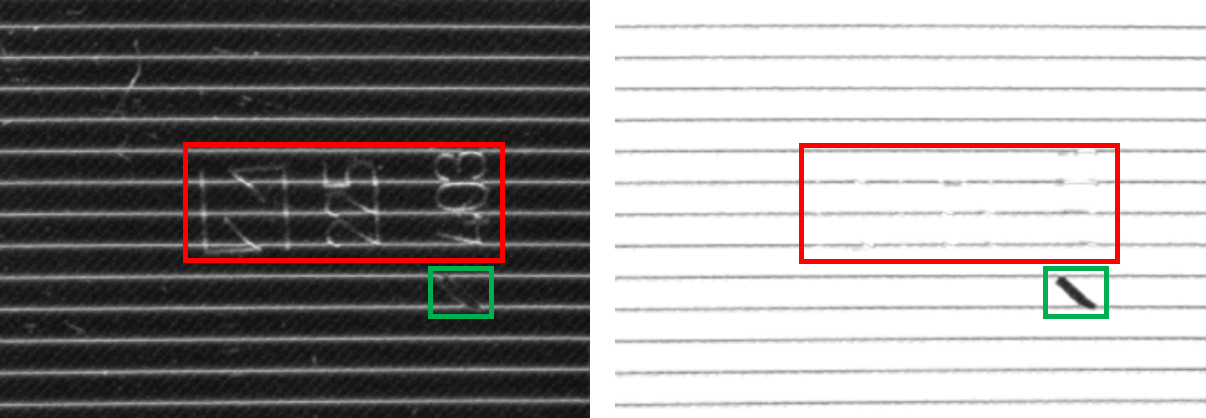
\includegraphics[width=\textwidth]{03_sichtpruefungDurchLichtstreuung/einsatzVonMehrerenStreifenmustern/figures/minAndMaxLink}
	\caption[Verknüpfte Bilder über Minimierung und Maximierung]{Verknüpfte Bilder um Defekte von \textit{Fall 1} (rot umrahmt) und Defekte von \textit{Fall 2} (grün umrahmt) isoliert voneinander zu betrachten. Links über Minimierung und rechts über Maximierung verknüpft.}
	\label{img:minAndMaxLink}
\end{figure}

\noindent
In diesen Bildern sind noch horizontale Streifen zu erkennen.
Diese sind keine Defekte, sondern entstehen aus Überlappungen der Streifenmuster in den Kamerabildern.
Auf diese \glqq Fehler\grqq ~und Möglichkeiten zur Beseitigung dieser wird im nächsten Abschnitt \ref{sec:optimierungen} ~eingegangen.

\p
Als Nächstes kann man eine Möglichkeit aufstellen, um beide Fälle in einem Gesamtbild kenntlich zu machen.
Hierfür macht man sich die Gemeinsamkeiten von \textit{Fall 1} und \textit{Fall 2} zunutze.
Man kann feststellen, dass die Helligkeit der Defekte in beiden Kamerabildern trotz Veränderung der Muster ungefähr gleich bleibt.
Das bedeutet, bildet man zur Verknüpfung der Bilder die betragsmäßige Differenz werden Defekte aus den beiden Fällen dunkel.
Die restliche, normal-spiegelnde Oberfläche wird hell, da jeder sonstige Bildpunkt in einem Muster dunkel und im anderen Muster hell erscheinen sollte, also eine hohe Differenz ergibt.
Die Ausnahme bilden dabei auch hier die Überlappungen von Streifen.

\begin{figure}[H]
	\centering
	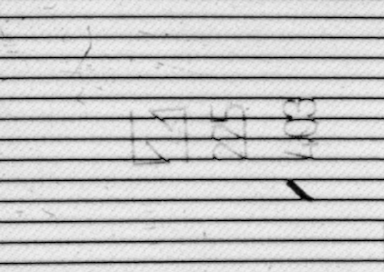
\includegraphics[width=0.5\textwidth]{03_sichtpruefungDurchLichtstreuung/einsatzVonMehrerenStreifenmustern/figures/diffImage}
	\caption[Verknüpfte Bilder über Differenz]{Über betragsmäßige Differenz verknüpfte Bilder.}
	\label{img:diffImage}
\end{figure}